% ============================================================
% UniBA Collab Thesis Template
% Versione 1.2.1
%
% Ideato, sviluppato e mantenuto da Giulio Mallardi
% Collab – Collaborative Development Group
% Dipartimento di Informatica
% Università degli Studi di Bari Aldo Moro
% https://collab.di.uniba.it/
%
% Copyright © 2025–2026 Giulio Mallardi
%
% Utilizzo e modifica consentiti secondo i termini contenuti
% nel file LICENSE.txt. È obbligatorio mantenere i crediti nei
% sorgenti e l’attribuzione visibile nel documento finale.
% ============================================================
\PassOptionsToPackage{table, dvipsnames}{xcolor}
\documentclass[a4paper,oneside,12pt]{toptesi}
\usepackage[T1]{fontenc}
\usepackage[utf8]{inputenc}
\usepackage[italian]{babel}
\usepackage{algorithm}
\usepackage{algpseudocode}
\floatname{algorithm}{Algoritmo}
\algtext*{EndIf}
\algtext*{EndFor}
\usepackage{placeins}
\usepackage{tikz}
\usepackage{booktabs}
\usepackage{tabularx}
\usepackage{float}
\usepackage{amsmath}
\numberwithin{algorithm}{chapter}
\usetikzlibrary{positioning}
\usepackage{pgfplots}
\usepackage[newfloat]{minted}
\usepackage[font=small,skip=1pt]{caption}
\usepackage{minted}
\usepackage{subcaption}
\pgfplotsset{compat=1.18}
\usepackage{xurl}
\usepackage{hyperref}
\hypersetup{
    colorlinks = true,
    allcolors=black,
    pdftitle={Sintesi di un algoritmo basato su ResNet per Windows PE malware detection},
    pdfauthor={Domenico Bianchini},
    pdfsubject={Tesi di laurea in Informatica},
    pdfkeywords={malware; Windows PE; Deep Learning; ResNet-50; malware detection}
}
%This equals 1.5 linespacing in Word
\linespread{1.25}

\usepackage{fancyhdr} % nel preambolo, se non già incluso
\usepackage{graphicx} % per il logo
\usepackage{ifthen}   % per i controlli condizionali (facoltativo ma utile)

\let\savedlisting\listing
\AtBeginDocument{\let\listing\savedlisting}


\def\dept{DIPARTIMENTO DI INFORMATICA}
\def\course{CORSO DI LAUREA IN INFORMATICA}
%\def\course{CORSO DI LAUREA IN INFORMATICA E \\ TECNOLOGIE PER LA PRODUZIONE DEL SOFTWARE}
%\def\course{CORSO DI LAUREA MAGISTRALE IN INFORMATICA}
%\def\course{CORSO DI LAUREA MAGISTRALE IN SICUREZZA INFORMATICA}
\def\title{Sintesi di un algoritmo basato su ResNet per Windows PE malware detection}
\def\author{Domenico Bianchini}
\def\relatoreone{Prof.ssa Annalisa Appice}
\def\relatoretwo{}
\def\correlatoreone{Prof.ssa Giuseppina Andresini}
\def\correlatoretwo{}
\def\subject{METODI AVANZATI DI PROGRAMMAZIONE}
\def\annoacc{2025 - 2026}
\def\beforecandidate{LAUREANDO:}
\def\beforetitle{TESI DI LAUREA \\ IN \\}
\def\beforeprof{RELATRICE:}
\def\beforecorrelatore{CORRELATRICE:}
\def\beforeannoacc{ANNO ACCADEMICO}

\makeatletter
\def\cleardoublepage{\clearpage\if@twoside \ifodd\c@page\else
    \hbox{}
    \vspace*{\fill}
    \vspace{\fill}
    \thispagestyle{empty}
    \newpage
    \if@twocolumn\hbox{}\newpage\fi\fi\fi}
\makeatother


\begin{document}

\raggedbottom

\begin{titlepage}
	\begin{tikzpicture}[remember picture,overlay]
		\centering
		\node[yshift=-6 cm] (logo) at (current page.north) {
\includegraphics[width=0.75\linewidth]{images/uniba.pdf}};
			\node[text width=50em,yshift=0.25cm, align = center, below = of logo](dipartimento){\Large \dept};
            	%\node[yshift=0.25 cm, align = center, below = of logo] (dipartimento)  {\includegraphics[width=0.75\linewidth]{images/dib.pdf}};
			\node[text width=40em, align = center, yshift=.55cm,below = of dipartimento](course){\normalsize \course};
		\node[text width=35em,align = center,  yshift=1.2cm,below = of course](line){\par\noindent\rule{\textwidth}{0.4pt}};
		\node[text width=40em, align = center, yshift=.55cm,below = of line](lia){\normalsize \beforetitle \xspace \subject };
		
  \node[text width=40em, align = center, yshift=-0.5cm,below = of lia](title){\bfseries \parbox{12cm}{\fontsize{21pt}{20pt}\selectfont \centering \title\par}};
  
	\node[text width=35em, align = left, yshift=-1cm,below = of title](relatoretit){\normalsize \textbf{\beforeprof} };
 	\node[text width=35em, align = left, yshift=1cm,below = of relatoretit](relatore){\large \relatoreone \\ \relatoretwo};

  	\node[text width=35em, align = left, yshift=0.5cm,below = of relatore](correlatoretit){\normalsize \textbf{\beforecorrelatore}  };
     \node[text width=35em, align = left, yshift=1cm,below = of correlatoretit](correlatore){\large \correlatoreone \\ \correlatoretwo};
      
		\node[text width=35em, align = right, yshift=-1cm,below = of title](candidatetit){\normalsize \textbf{\beforecandidate}};
		 \node[text width=35em, align = right, yshift=1cm,below = of candidatetit](candidate){\large \author};

  \node[text width=35em,align = center,  yshift= -3cm,below = of candidate](line2){\par\noindent\rule{\textwidth}{0.4pt}};
	
  
  \node[text width=50em, align = center, yshift=0.5cm,below = of line2](year){\large \beforeannoacc\xspace \annoacc};
	\end{tikzpicture}
\end{titlepage}


\cleardoublepage

% \begin{dedication}
    \begin{flushright}
        {\small % Cambia la dimensione del font qui
        \textit{``A volte sono le persone che nessuno immagina possano fare certe cose,\\
        a fare cose che nessuno può immaginare.'' \\ 
        --- Alan Turing, The Imitation Game \\[2em]
        \footnotesize Dedico questo lavoro a me stesso}}
    \end{flushright}
\end{dedication}
% \cleardoublepage

\pagenumbering{roman}

% \chapter*{Disclaimer}
Tutti i marchi, nomi commerciali, prodotti e loghi menzionati in questo elaborato sono di proprietà dei rispettivi titolari. 
L’autore non rivendica alcun diritto su tali marchi o nomi commerciali e li utilizza esclusivamente a scopo informativo e descrittivo, senza alcun intento di violazione.

% --- Definizione del footer personalizzato per il Disclaimer ---
\fancypagestyle{collabfooter}{
  \fancyhf{} % pulisce header e footer
  \fancyfoot[C]{%
      \vspace{-3cm} % alza il footer di circa 1 cm

    \IfFileExists{images/collab.pdf}{%
      
\includegraphics[width=2.2cm]{images/collab.pdf}\\[12pt]
    }{}%
    {\scriptsize
      Questa tesi è stata realizzata nell’ambito delle attività di ricerca del\\ 
        \textbf{}\\
      \textbf{Collab – Collaborative Development Group}\\ 
        https://collab.di.uniba.it/ \\
      Dipartimento di Informatica, Università degli Studi di Bari Aldo Moro
    }%
  }
  \renewcommand{\headrulewidth}{0pt}
  \renewcommand{\footrulewidth}{0pt} % linea sottile sopra il footer (facoltativa)
}

\thispagestyle{collabfooter}

% \cleardoublepage

\tableofcontents
\cleardoublepage

\pagenumbering{arabic}
\setcounter{page}{1}

\chapter{Introduzione}

\section{Contesto e motivazioni}

\section{Obiettivi della tesi}

\section{Struttura della tesi}
\chapter{Malware e file Windows PE}

\section{Il formato Windows PE}

Il Portable Executable (PE) è il formato utilizzato nei sistemi Windows
per i file \texttt{.exe}, \texttt{.dll} e altre tipologie di file
eseguibili. Inizialmente progettato come formato eseguibile standard
per i sistemi Windows, il formato PE, fin dalla sua introduzione, ha
subito diverse modifiche, anche in seguito al passaggio ai sistemi
Windows a 64 bit.

La struttura di un file PE contiene le informazioni necessarie al
sistema operativo Windows per caricare e gestire il codice eseguibile.
Oltre al codice da eseguire, un file PE contiene infatti metadati e
altre informazioni organizzate secondo una struttura ben definita,
la cui conoscenza riveste un ruolo importante nell'ambito dell'analisi
dei malware.

In particolare, la struttura di un file PE è organizzata in tre parti
principali \cite{microsoftPE}, come mostrato nella
Figura~\ref{fig:pe_structure}:

\begin{itemize}
    \item \textbf{Header}: contiene le informazioni principali relative
    al file PE e al suo caricamento in memoria. L'header è a sua volta
    suddiviso nelle seguenti parti:

    \vspace{-0.5em}
    \begin{itemize}
        \item \textbf{DOS Header}: rappresenta la parte iniziale del file PE
        e contiene informazioni relative al formato DOS. Contiene inoltre un
        riferimento che indica la posizione iniziale del PE Header;

        \item \textbf{DOS Stub}: viene utilizzato per visualizzare un messaggio
        che indica se il programma può essere eseguito o meno in modalità DOS;

        \item \textbf{NT Header}: contiene le principali informazioni
        relative al file PE ed è a sua volta suddiviso in:

        \begin{itemize}
            \item \textbf{PE Signature}: identifica il file come Portable
            Executable;

            \item \textbf{COFF File Header}: contiene informazioni sulle
            caratteristiche del file e sulle sezioni presenti;

            \item \textbf{Optional Header}: contiene informazioni utilizzate
            durante il caricamento del file in memoria, tra cui il punto di
            ingresso del programma.
        \end{itemize}
    \end{itemize}

    \item \textbf{Tabella delle sezioni}: descrive le caratteristiche delle
    diverse sezioni presenti nel file e contiene le informazioni necessarie
    per mapparle in memoria e indicare se ciascuna sezione è di sola lettura
    oppure scrivibile;

    \item \textbf{Sezioni}: contengono il codice e i dati del file PE.
    Tra le sezioni comunemente presenti si trovano:

    \begin{itemize}
        \item \texttt{.text}: contiene il codice eseguibile;

        \item \texttt{.data}: contiene le variabili globali e statiche
        inizializzate;

        \item \texttt{.bss}: contiene le variabili globali e statiche
        non inizializzate;

        \item \texttt{.rsrc}: contiene le risorse utilizzate dal programma,
        come icone, immagini, stringhe e finestre di dialogo;

        \item \texttt{.reloc}: contiene i dati necessari alla rilocazione
        del programma;
    \end{itemize}
\end{itemize}

\begin{figure}[!ht]
    \centering
    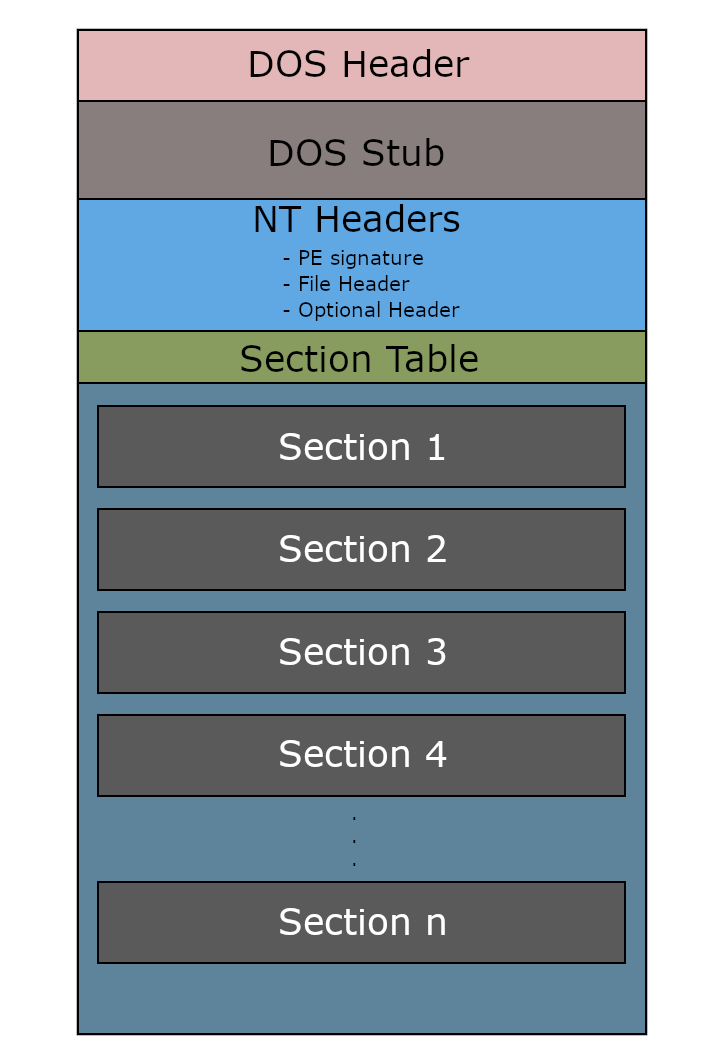
\includegraphics[width=0.6\textwidth]{images/pe_structure.png}
    \caption{Struttura generale di un file PE, tratta da \cite{khan2023}}
    \label{fig:pe_structure}
\end{figure}

\FloatBarrier

L'header riveste un ruolo importante nella classificazione dei malware,
dato che le informazioni in esso contenute sono risultate tra quelle
che contribuiscono maggiormente al processo di classificazione
\cite{zhang2024}.

L'analisi della struttura delle sezioni può essere utile anche
nell'ambito del rilevamento dei malware, dato che il codice malevolo
può essere nascosto all'interno di sezioni insolite oppure possono
essere aggiunte ulteriori sezioni con l'obiettivo di rendere più
complessa l'analisi del file. Inoltre, i file malware possono presentare
anomalie nella struttura e nelle caratteristiche del formato PE rispetto
ai file benigni, rendendo queste informazioni rilevanti per il loro
rilevamento \cite{bai2014}.

\vspace{0.5cm}

\section{Malware e tecniche di rilevamento}

Il termine malware deriva da \textit{malicious software} e indica
un software progettato con lo scopo di compromettere la riservatezza,
l'integrità o la disponibilità dei dati, delle applicazioni o del
sistema operativo \cite{souppaya2013}.

I malware possono essere suddivisi in diverse tipologie in base alle
loro caratteristiche e al loro comportamento. Inoltre, queste categorie
non sono esclusive, poiché uno stesso malware può presentare
contemporaneamente caratteristiche appartenenti a più tipologie
\cite{egele2012}.

Tra le principali tipologie di malware abbiamo i \textit{worm}, che
sono programmi in grado di essere eseguiti in modo indipendente e con
la capacità di propagarsi verso altri sistemi. I worm possono inoltre
essere utilizzati per creare \textit{botnet}, impiegate per l'invio
di messaggi di spam o per effettuare attacchi di tipo Distributed
Denial of Service (DDoS), nei quali più computer infettati da worm
agiscono in modo coordinato per esaurire le risorse di un sistema o
la sua banda di rete.

I \textit{virus}, a differenza dei worm, non possono essere eseguiti
in modo indipendente, ma inseriscono il proprio codice malevolo
all'interno di altri programmi e si attivano quando viene eseguito
il programma infettato. Possono inoltre propagarsi infettando altri
file presenti nel sistema e, attraverso file presenti su server
condivisi, diffondersi anche verso altri computer.

I \textit{Trojan horse} sono programmi che si presentano come software
legittimi, ma che eseguono operazioni malevole in background. Una volta
installati, possono ad esempio scaricare altri malware, modificare le
impostazioni del sistema o infettare altri file.

Gli \textit{spyware} sono malware utilizzati per raccogliere informazioni
sensibili dal sistema infetto e trasmetterle all'attaccante. Le
informazioni raccolte possono comprendere credenziali di accesso,
dati bancari, pagine web visitate oppure il contenuto di documenti
ed e-mail.

I \textit{bot} permettono a un attaccante, chiamato \textit{bot master},
di controllare da remoto il sistema infetto. Un insieme di bot
controllati dallo stesso \textit{bot master} costituisce una
\textit{botnet}, che può essere utilizzata, ad esempio, per l'invio
di messaggi di spam o per attività di spyware.

Infine, i \textit{rootkit}, la cui principale caratteristica è quella
di nascondere determinate informazioni all'utente del sistema, come
processi, file o connessioni di rete. Per questo motivo, molti malware
utilizzano tecniche proprie dei rootkit per nascondere la propria
presenza all'interno del sistema.

Il rilevamento dei malware può essere effettuato attraverso diverse
tecniche. Uno degli approcci tradizionalmente utilizzati, anche dagli
antivirus, è quello basato sulle firme, in cui i file vengono confrontati
con un insieme di firme associate a malware già conosciuti.

Questo approccio presenta tuttavia alcuni limiti, in particolare le firme
vengono generalmente create da analisti, richiedendo tempo e potendo
essere soggette a errori. Inoltre, i metodi basati sulle firme non sono
in grado di rilevare minacce sconosciute per le quali non è ancora
disponibile una firma, dato che solo quando viene individuata una nuova
minaccia questa può essere analizzata e può essere creata una nuova
firma, che viene successivamente aggiunta al database utilizzato per
il rilevamento \cite{egele2012}.

Per affrontare alcuni dei limiti dei metodi basati sulle firme, sono
state sviluppate altre tecniche per il rilevamento dei malware. In
particolare, è possibile distinguere due principali approcci:
l'analisi dinamica e l'analisi statica, in base all'esecuzione o meno
del programma durante la raccolta delle feature, ovvero delle
caratteristiche utilizzate per effettuare l'analisi
\cite{zhang2024}.

\begin{figure}[!ht]
    \centering

    \begin{tikzpicture}[
        node distance=0.7cm and 1.2cm,
        main/.style={
            draw,
            rounded corners=2pt,
            align=center,
            minimum height=0.9cm,
            text width=4.2cm
        },
        title/.style={
            draw,
            rounded corners=2pt,
            align=center,
            minimum height=0.9cm,
            text width=4.2cm,
            font=\bfseries
        },
        arrow/.style={
            -{Latex[length=2mm]},
            thick
        }
    ]

        % Titolo
        \node[title] (analysis)
        {Analisi dei malware};

        % Due approcci
        \node[title, below left=0.8cm and 0.7cm of analysis]
        (dynamic)
        {Analisi dinamica};

        \node[title, below right=0.8cm and 0.7cm of analysis]
        (static)
        {Analisi statica};

        % Esecuzione
        \node[main, below=of dynamic]
        (dynamicExecution)
        {Programma in esecuzione};

        \node[main, below=of static]
        (staticExecution)
        {Programma non eseguito};

        % Informazioni analizzate
        \node[main, below=of dynamicExecution]
        (dynamicInformation)
        {Comportamento del programma};

        \node[main, below=of staticExecution]
        (staticInformation)
        {Contenuto del file};

        % Feature
        \node[main, below=of dynamicInformation]
        (dynamicFeatures)
        {Chiamate API\\
        Comunicazioni di rete\\
        Memoria e CPU};

        \node[main, below=of staticInformation]
        (staticFeatures)
        {Rappresentazione binaria};

        % Frecce
        \draw[arrow] (analysis) -- (dynamic);
        \draw[arrow] (analysis) -- (static);

        \draw[arrow] (dynamic) -- (dynamicExecution);
        \draw[arrow] (static) -- (staticExecution);

        \draw[arrow] (dynamicExecution) -- (dynamicInformation);
        \draw[arrow] (staticExecution) -- (staticInformation);

        \draw[arrow] (dynamicInformation) -- (dynamicFeatures);
        \draw[arrow] (staticInformation) -- (staticFeatures);

    \end{tikzpicture}

    \caption{Confronto tra analisi dinamica e analisi statica dei malware,
    basato su \cite{zhang2024}}
    \label{fig:static_dynamic_analysis}
\end{figure}

L'analisi dinamica prevede l'esecuzione del programma e l'osservazione
del suo comportamento durante l'esecuzione. In questo modo possono
essere raccolte diverse informazioni, tra cui le sequenze delle
chiamate API, le comunicazioni di rete, lo stato della memoria e
della CPU. Questo tipo di analisi può inoltre contribuire al
rilevamento di malware precedentemente sconosciuti e risulta meno
vulnerabile alle tecniche di offuscamento del codice. 

Tuttavia, presenta alcuni limiti, dato che ogni campione deve essere
eseguito per un determinato periodo di tempo e può essere analizzato
un singolo percorso di esecuzione del programma \cite{bai2014}.

A differenza dell'analisi dinamica, l'analisi statica permette di
analizzare un programma senza eseguirlo e, per questo motivo, richiede
tempi inferiori per l'analisi. Dato che generalmente il codice sorgente
dei malware non è disponibile, le tecniche di analisi statica
applicabili devono ricavare le informazioni direttamente dalla
rappresentazione binaria del programma.

Anche l'analisi statica presenta alcuni limiti, dato che lavorare
direttamente sulla rappresentazione binaria di un programma può
risultare complesso. Inoltre, i malware possono utilizzare tecniche
in grado di modificare il programma e ostacolare questo tipo di
analisi \cite{egele2012}.

I limiti degli approcci descritti in precedenza, insieme alla crescente
complessità e quantità dei malware, hanno favorito l'utilizzo di
tecniche basate sul Machine Learning. In particolare, queste tecniche
permettono di apprendere modelli e pattern a partire dalle feature
estratte dai malware, con l'obiettivo di supportarne il rilevamento
e l'analisi \cite{ucci2019}.
\chapter{Scoperta di Windows PE malware}

\section{Conversione di file PE in immagini}

\section{ResNet per classificazione di immagini}
\chapter{Validazione empirica}

\section{Dataset}

Per la validazione sperimentale è stato utilizzato il
\textit{PE Malware Machine Learning Dataset} di Practical Security
Analytics \cite{lester2021}. Il dataset comprende, oltre ai file PE,
un file CSV contenente diverse informazioni associate a ciascun
file, tra cui la lunghezza in byte e l'etichetta che indica
l'appartenenza alla \textit{Whitelist} o alla \textit{Blacklist},
permettendo di distinguere rispettivamente i file benigni da quelli
malevoli. Queste caratteristiche rendono il dataset particolarmente
adatto al lavoro svolto, poiché mette a disposizione sia i file PE
originali, necessari per la loro conversione in immagini, sia le
relative etichette utilizzate per la classificazione.

Il dataset è composto complessivamente da 201.549 file PE, di cui
86.812 appartenenti alla \textit{Whitelist} e quindi considerati
benigni, e 114.737 appartenenti alla \textit{Blacklist} e quindi
considerati malevoli.

Ai fini della validazione sperimentale, il dataset è stato suddiviso
in un training set, contenente l'80\% dei campioni, e un test set,
contenente il restante 20\%. La suddivisione è stata effettuata in
modo stratificato rispetto alla classe, così da mantenere la
proporzione tra file benigni e malevoli presente nel dataset
originale.

\begin{table}[!ht]
    \centering
    \caption{Distribuzione dei campioni nei set di training e test}
    \label{tab:dataset_split}
    \renewcommand{\arraystretch}{1.3}
    \begin{tabular}{lrrr}
        \toprule
        \textbf{Insieme} & \textbf{Benigni} & \textbf{Malevoli}
        & \textbf{Totale} \\
        \midrule
        Training & 69.450 & 91.789 & 161.239 \\
        Test     & 17.362 & 22.948 & 40.310 \\
        \midrule
        Totale   & 86.812 & 114.737 & 201.549 \\
        \bottomrule
    \end{tabular}
\end{table}

Il training set è stato utilizzato per l'addestramento del modello,
mentre il test set è stato utilizzato per valutarne le prestazioni,
dato che contiene dati non utilizzati durante il training e quindi
permette di valutare il modello su campioni mai utilizzati durante
l'addestramento.

\section{Set-up e metriche}



\section{Risultati}
\chapter{Conclusioni e sviluppi futuri}

In questo lavoro di tesi è stato affrontato il problema della classificazione
di file Windows PE come benigni o malevoli attraverso la loro
rappresentazione sotto forma di immagini e tramite l'utilizzo di una rete
ResNet-50. In particolare, sono state confrontate le strategie di
mapping LINEAR, ZIGZAG e SERPENTINE, considerando sia immagini RGB
sia immagini in scala di grigi e le due diverse strategie relative alle
dimensioni, a dimensione fissa e ad altezza variabile.
Nel complesso, i risultati ottenuti hanno mostrato prestazioni
elevate per tutte le configurazioni considerate, evidenziando
risultati migliori per le configurazioni ad altezza variabile
rispetto alle corrispondenti configurazioni a dimensione fissa.
In particolare, la migliore overall accuracy è stata ottenuta
dalla configurazione SERPENTINE RGB ad altezza variabile, con un
valore pari al 97,61\%.
L'approccio basato sulla rappresentazione dei file PE come immagini
e sulla loro classificazione mediante ResNet-50 ha permesso di
ottenere buone prestazioni sul dataset considerato, mostrando inoltre
come la scelta delle dimensioni delle immagini possa avere un ruolo
importante nelle prestazioni del modello.

Come possibile sviluppo futuro, l'analisi potrebbe essere estesa
utilizzando dataset differenti, in modo da verificare se le
prestazioni rimangano coerenti anche su altri insiemi di file PE.
Un ulteriore sviluppo potrebbe riguardare il confronto
\textcolor{red}{della accuratezza della classificazione ottenuta con la} rete
ResNet-50 \textcolor{red}{con l'accuratezza che si potrebbe ottenere usando} altre architetture della stessa
famiglia, caratterizzate da una diversa profondità, in modo da
valutare l'influenza del numero di livelli sulle prestazioni ottenute.
Potrebbero inoltre essere valutate diverse modalità per determinare
le dimensioni delle immagini, ad esempio calcolandole in funzione
della lunghezza in byte del singolo file PE, invece di utilizzare
una larghezza comune determinata a partire dalla lunghezza media in
byte dei file del dataset.
\textcolor{red}{Nella versione attuale della tesi, la fase di pre-elaborazione}
delle immagini, \textcolor{red}{compresa la fase di ridimensionamento (resize)}
\textcolor{red}{delle immagini, sono state, entrambe, eseguite} prima di fornire
le immagini in input alla ResNet-50, mentre potrebbe essere interessante valutare come cambiano
le prestazioni utilizzando l'AutoImageProcessor di Hugging Face
\cite{huggingface_autoimageprocessor} per la preparazione delle
immagini.
Questi possibili sviluppi permetterebbero di proseguire l'analisi e
approfondire \textcolor{red}{, in futuro, come la} rappresentazione dei file PE come
immagini \textcolor{red}{possa contribuire a migliorare l'accuratezza della} classificazione di file benigni e malevoli.

\appendix
\chapter{Progettazione UML}

\section{Diagramma UML generale}

Il diagramma riportato nella Figura~\ref{fig:uml_general} mostra la
struttura complessiva del progetto, evidenziando le classi, i package di
appartenenza e le relazioni tra le classi.

\begin{figure}[H]
    \centering
    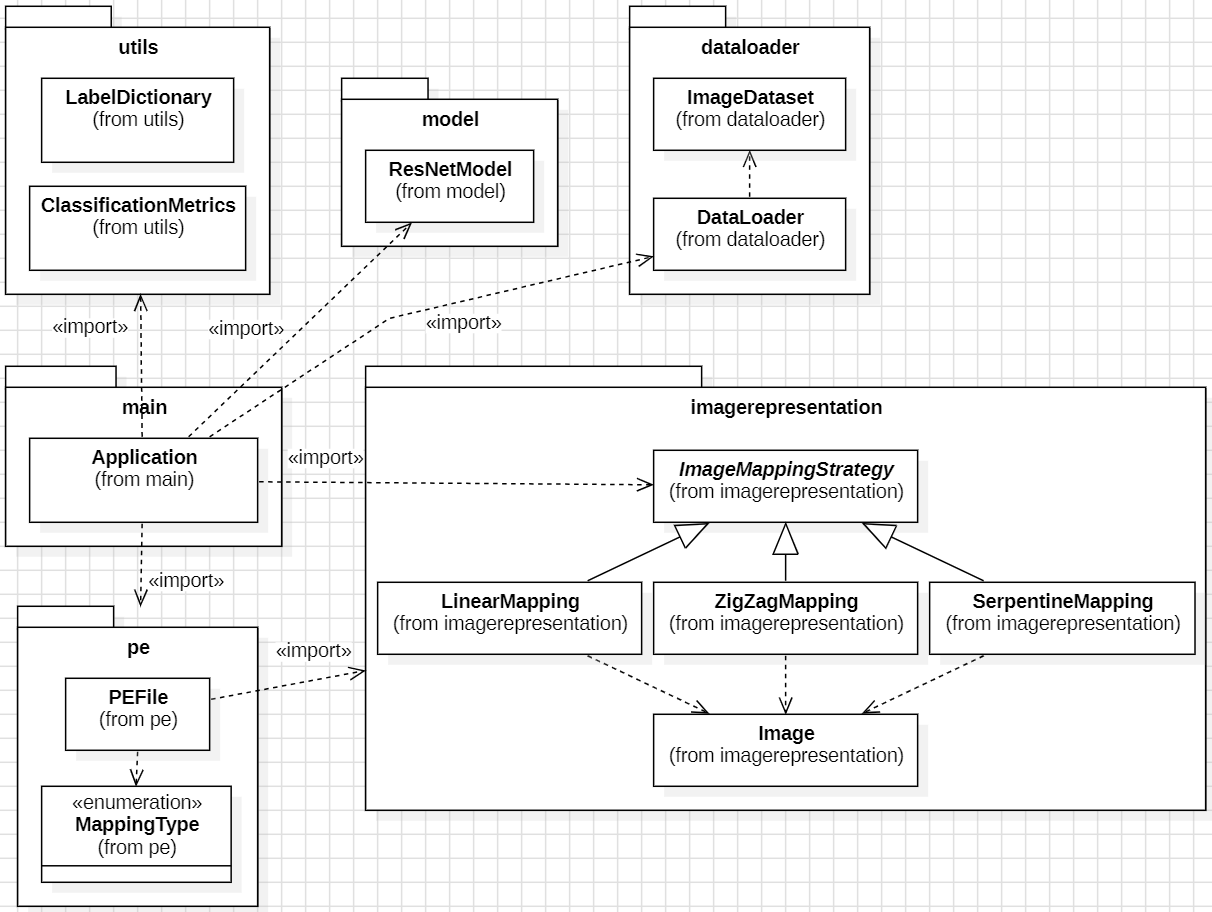
\includegraphics[width=0.971\textwidth]{images/uml_general.png}
    \caption{Diagramma UML generale del progetto}
    \label{fig:uml_general}
\end{figure}

\section{Package main}

Il package \texttt{main} (Figura~\ref{fig:package_main}) contiene il
punto di ingresso del programma e coordina l’esecuzione della pipeline.
Al suo interno vengono letti i parametri del file di configurazione e
vengono avviate le principali fasi del processo.

\begin{figure}[H]
    \centering
    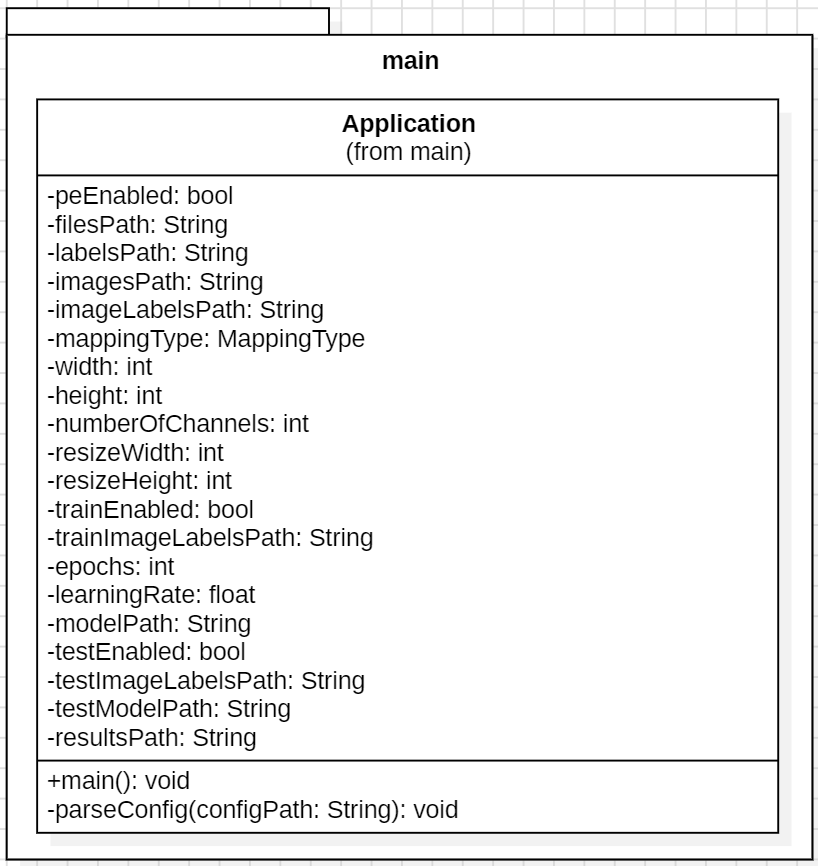
\includegraphics[width=0.85\textwidth]{images/package_main.png}
    \caption{Diagramma UML del package \texttt{main}}
    \label{fig:package_main}
\end{figure}

\subsection{Classe Application}

La classe \texttt{Application}, appartenente al package \texttt{main}, è
la classe principale del programma e si occupa di leggere il file di
configurazione e, in base ai parametri
impostati, di coordinarne le diverse fasi. Per svolgere le
varie operazioni, richiama le classi responsabili della conversione dei
file PE, della creazione del file CSV con le etichette, del training e
del test del modello. Durante la fase di test, coordina anche il calcolo
delle metriche e il salvataggio dei risultati.

\paragraph{Attributi}

\begin{itemize}
    \raggedright
    \item \textbf{peEnabled} (\texttt{bool}): indica se abilitare la fase di
    conversione PE in immagini.
    \item \textbf{filesPath} (\texttt{String}): percorso della cartella
    contenente i file PE da convertire.
    \item \textbf{labelsPath} (\texttt{String}): percorso del file CSV
    contenente i nomi dei file PE e le relative etichette.
    \item \textbf{imagesPath} (\texttt{String}): percorso della cartella in cui
    vengono salvate le immagini generate.
    \item \textbf{imageLabelsPath} (\texttt{String}): percorso del file CSV
    in cui viene salvato il mapping tra il percorso delle immagini generate e
    le relative etichette.
    \item \textbf{mappingType} (\texttt{MappingType}): strategia di mapping da
    utilizzare.
    \item \textbf{width} (\texttt{int}): larghezza delle immagini da generare.
    \item \textbf{height} (\texttt{int}): altezza delle immagini da generare.
    \item \textbf{numberOfChannels} (\texttt{int}): numero di canali
    delle immagini da generare.
    \item \textbf{resizeWidth} (\texttt{int}): larghezza per l'eventuale resize.
    \item \textbf{resizeHeight} (\texttt{int}): altezza per l'eventuale resize.
    \item \textbf{trainEnabled} (\texttt{bool}): indica se abilitare la fase di
    training del modello.
    \item \textbf{trainImageLabelsPath} (\texttt{String}): percorso del file CSV
    contenente il mapping immagini-etichette utilizzato durante il training.
    \item \textbf{epochs} (\texttt{int}): numero di epoche del training.
    \item \textbf{learningRate} (\texttt{float}): learning rate utilizzato
    durante il training.
    \item \textbf{modelPath} (\texttt{String}): percorso della cartella in cui
    viene salvato il modello addestrato.
    \item \textbf{testEnabled} (\texttt{bool}): indica se abilitare la fase di
    test del modello addestrato.
    \item \textbf{testImageLabelsPath} (\texttt{String}): percorso del file CSV
    contenente il mapping immagini-etichette utilizzato durante il test.
    \item \textbf{testModelPath} (\texttt{String}): percorso della cartella
    contenente il modello da utilizzare durante il test.
    \item \textbf{resultsPath} (\texttt{String}): percorso del file CSV in cui
    vengono salvati i risultati del test e le metriche calcolate.
\end{itemize}

\paragraph{Metodi}

\begin{itemize}
    \raggedright
    \item \textbf{main()} $\rightarrow$ \texttt{void}: punto di ingresso
    del programma. Coordina l’esecuzione delle diverse fasi in base ai
    parametri caricati dal file di configurazione.
    \item \textbf{parseConfig}(\texttt{configPath: String})
    $\rightarrow$ \texttt{void}: metodo
    privato che legge il file di configurazione e inizializza gli
    attributi necessari per l’esecuzione delle diverse fasi del programma.
\end{itemize}

\section{Package pe}

Il package \texttt{pe} (Figura~\ref{fig:package_pe}) si occupa della gestione dei file Portable
Executable di Windows. Il suo compito principale è leggere i file PE in
formato binario e avviare il processo di conversione in immagini,
utilizzando la strategia di mapping ricevuta dalla classe \texttt{Application}.

\begin{figure}[H]
    \centering
    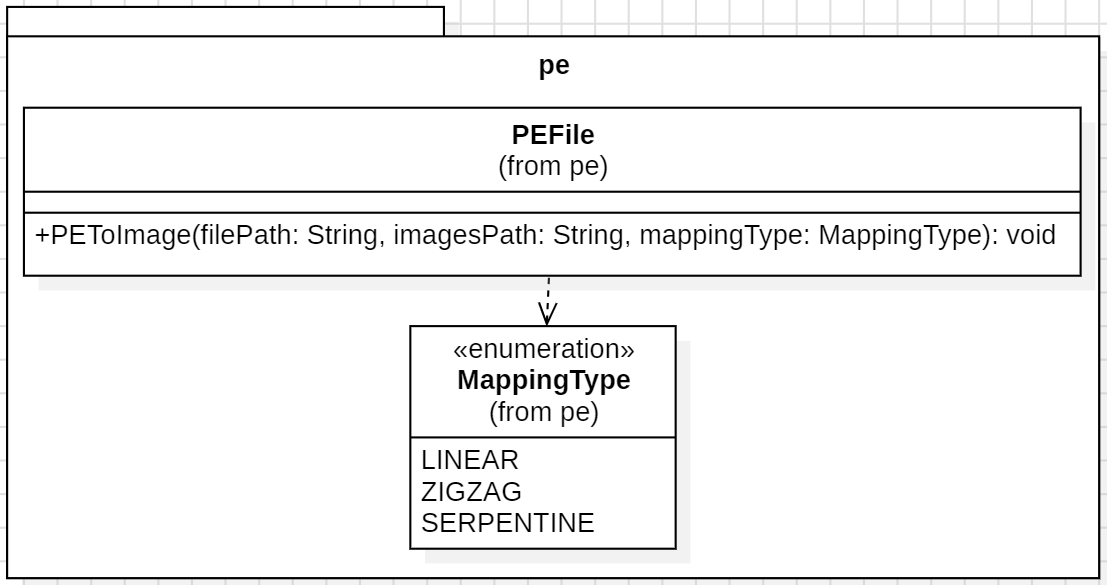
\includegraphics[width=\textwidth]{images/package_pe.PNG}
    \caption{Diagramma UML del package \texttt{pe}}
    \label{fig:package_pe}
\end{figure}

\subsection{Classe PEFile}

La classe \texttt{PEFile}, appartenente al package \texttt{pe}, è
responsabile della conversione di un singolo file PE. Riceve il percorso
del file, il percorso della cartella in cui
salvare l’immagine e il valore di \texttt{MappingType}. Dopo aver letto il
contenuto binario del file, utilizza il tipo di mapping ricevuto per
individuare la strategia da applicare e salva infine l’immagine generata
nella cartella specificata.

\paragraph{Metodi}

\begin{itemize}
    \raggedright
    \item \textbf{PEToImage}(\texttt{filePath:String},
    \texttt{imagesPath:String}, \texttt{mappingType:MappingType})
    $\rightarrow$ \texttt{void}: legge il singolo file PE indicato,
    genera l’immagine utilizzando la strategia di mapping ricevuta e salva
    il risultato nella cartella delle immagini specificata.
\end{itemize}

\subsection{Enumerazione MappingType}

L’enumerazione \texttt{MappingType}, appartenente al package \texttt{pe},
definisce il tipo di strategia di mapping da utilizzare per la conversione
dei file PE in immagini. Il valore viene letto dal file di configurazione
dalla classe
\texttt{Application} e passato alla classe
\texttt{PEFile}, che lo utilizza per determinare la strategia di mapping
da applicare durante la generazione delle immagini.

\paragraph{Valori}

\begin{itemize}
    \raggedright
    \item \textbf{LINEAR}
    \item \textbf{ZIGZAG}
    \item \textbf{SERPENTINE}
\end{itemize}

\section{Package image\_representation}

Il package \texttt{image\_representation} contiene le funzionalità
necessarie per la conversione dei file PE in immagini. Al suo interno
sono definite le diverse strategie di mapping utilizzate per disporre i
byte del file nell’immagine.

\begin{figure}[H]
    \centering
    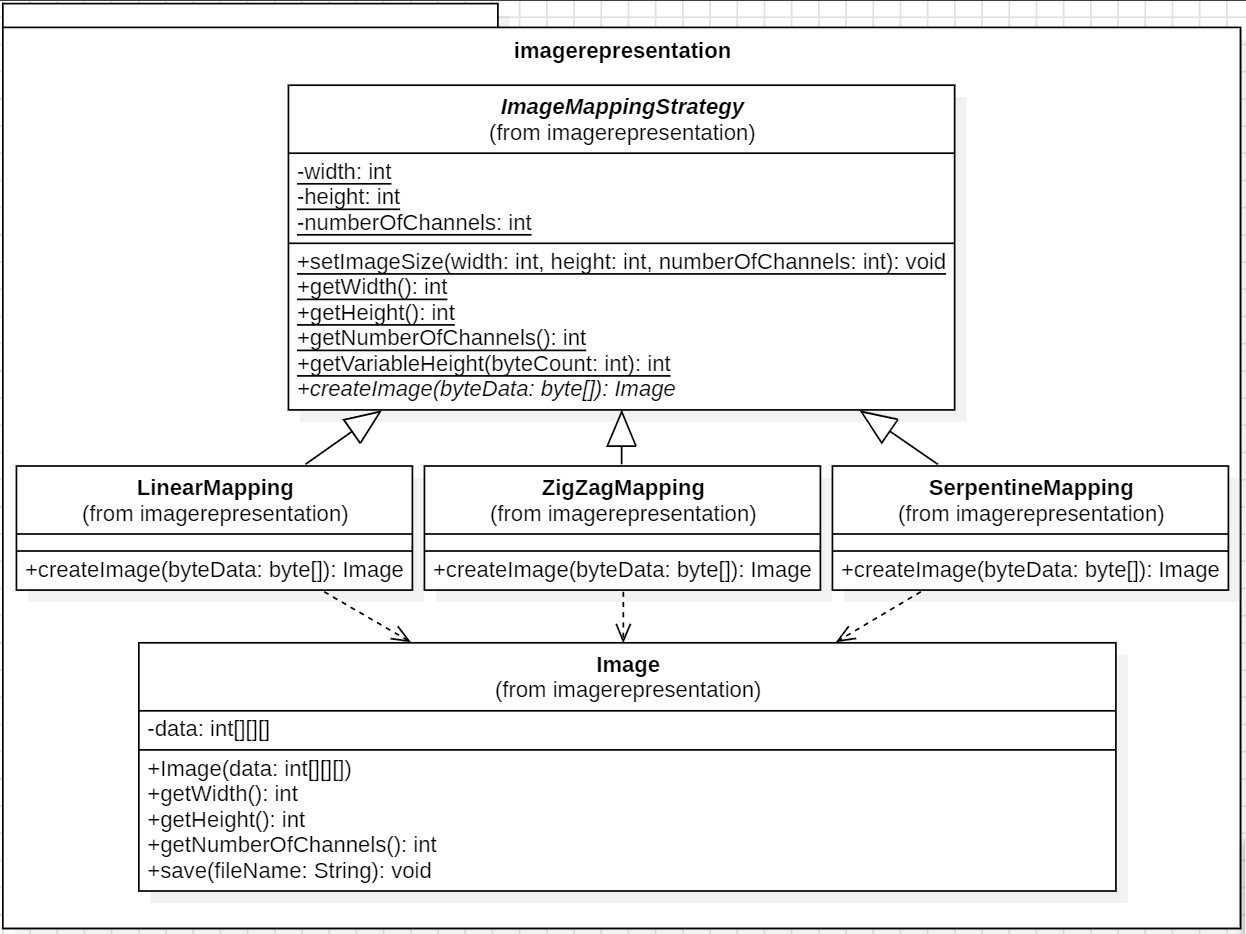
\includegraphics[width=\textwidth]{images/package_imagerepresentation.PNG}
    \caption{Diagramma UML del package \texttt{image\_representation}}
    \label{fig:package_image_representation}
\end{figure}

\subsection{Classe Image}

La classe \texttt{Image}, appartenente al package
\texttt{image\_representation}, rappresenta l’immagine finale ottenuta
dalla conversione del file PE. L’immagine è rappresentata tramite un tensore a
tre dimensioni che contiene i valori dei pixel organizzati secondo righe,
colonne e canali. La classe riceve il tensore già costruito dalla strategia
di mapping e si occupa della sua gestione e del salvataggio su file.

\paragraph{Attributi}

\begin{itemize}
    \raggedright
    \item \textbf{data} (\texttt{int[][][]}): tensore tridimensionale che
    contiene i valori dell’immagine organizzati in altezza, larghezza e
    numero di canali.
\end{itemize}

\paragraph{Metodi}

\begin{itemize}
    \raggedright
    \item \textbf{Image}(\texttt{data:int[][][]}): costruttore della classe
    che inizializza l’immagine.
    \item \textbf{getWidth}() $\rightarrow$ \texttt{int}: restituisce la
    larghezza dell’immagine ricavandola dal tensore associato.
    \item \textbf{getHeight}() $\rightarrow$ \texttt{int}: restituisce
    l’altezza dell’immagine ricavandola dal tensore associato.
    \item \textbf{getNumberOfChannels}() $\rightarrow$ \texttt{int}:
    restituisce il numero di canali dell’immagine ricavandola dal tensore
    associato.
    \item \textbf{save}(\texttt{fileName:String}) $\rightarrow$
    \texttt{void}: salva l’immagine su file.
\end{itemize}

\subsection{Classe astratta ImageMappingStrategy}

La classe astratta \texttt{ImageMappingStrategy} definisce il comportamento
comune delle strategie di mapping. Appartiene al package
\texttt{image\_representation}. Contiene i parametri necessari alla
costruzione dell’immagine, cioè larghezza, altezza e numero di canali,
impostati prima della fase di creazione dell’immagine. Ogni implementazione
riceve in input la sequenza di byte del file PE e costruisce l’immagine
utilizzando un diverso ordine di inserimento dei dati in base alla strategia
scelta.
L’altezza può essere definita nel file di configurazione oppure impostata a
0 per utilizzare la modalità a altezza variabile. In questo caso, l’altezza
necessaria viene calcolata durante la creazione dell’immagine senza
modificare la configurazione della strategia.
La gestione dei canali permette di costruire immagini sia in grayscale
(1 canale) sia RGB (3 canali), modificando la granularità con cui i byte
vengono letti e inseriti nel tensore, in particolare un byte per pixel nel
caso grayscale oppure gruppi di tre byte per pixel nel caso RGB.

\paragraph{Attributi}

\begin{itemize}
    \raggedright
    \item \textbf{width} (\texttt{int}, statico): larghezza comune
    utilizzata per la costruzione delle immagini.
    \item \textbf{height} (\texttt{int}, statico): altezza comune
    utilizzata per la costruzione delle immagini.
    \item \textbf{numberOfChannels} (\texttt{int}, statico): numero di
    canali utilizzato per definire la struttura del tensore.
\end{itemize}

\paragraph{Metodi}

\begin{itemize}
    \raggedright
    \item \textbf{setImageSize}(\texttt{width:int}, \texttt{height:int},
    \texttt{numberOfChannels:int}) $\rightarrow$ \texttt{void}
    (statico): imposta i parametri comuni utilizzati dalle strategie per
    costruire l’immagine.
    \item \textbf{getVariableHeight}(\texttt{byteCount:int})
    $\rightarrow$ \texttt{int} (statico): calcola e restituisce l’altezza
    necessaria in base alla dimensione del file quando l’altezza non è
    definita.
    \item \textbf{getWidth}() $\rightarrow$ \texttt{int} (statico):
    restituisce la larghezza configurata.
    \item \textbf{getHeight}() $\rightarrow$ \texttt{int} (statico):
    restituisce l’altezza configurata.
    \item \textbf{getNumberOfChannels}() $\rightarrow$ \texttt{int}
    (statico): restituisce il numero di canali configurato.
    \item \textbf{createImage}(\texttt{byteData:byte[]}) $\rightarrow$
    \texttt{Image} (astratto): costruisce e restituisce l’immagine a partire
    dai byte del file PE.
\end{itemize}

\subsection{Classe LinearMapping}

La classe \texttt{LinearMapping}, appartenente al package
\texttt{image\_representation}, implementa il mapping inserendo i byte nel
tensore in modo sequenziale, da sinistra verso destra e dall’alto
verso il basso.

\paragraph{Metodi}

\begin{itemize}
    \raggedright
    \item \textbf{createImage}(\texttt{byteData:byte[]}) $\rightarrow$
    \texttt{Image}: costruisce l’immagine utilizzando il mapping lineare.
\end{itemize}

\subsection{Classe ZigZagMapping}

La classe \texttt{ZigZagMapping}, appartenente al package
\texttt{image\_representation}, implementa il mapping alternando la
direzione di riempimento delle righe, seguendo un andamento a zigzag.

\paragraph{Metodi}

\begin{itemize}
    \raggedright
    \item \textbf{createImage}(\texttt{byteData:byte[]}) $\rightarrow$
    \texttt{Image}: costruisce l’immagine utilizzando il mapping a zigzag.
\end{itemize}

\subsection{Classe SerpentineMapping}

La classe \texttt{SerpentineMapping}, appartenente al package
\texttt{image\_representation}, implementa il mapping seguendo un
andamento a serpentina.

\paragraph{Metodi}

\begin{itemize}
    \raggedright
    \item \textbf{createImage}(\texttt{byteData:byte[]}) $\rightarrow$
    \texttt{Image}: costruisce l’immagine utilizzando il mapping a
    serpentina.
\end{itemize}


\phantomsection
\bibliographystyle{unsrt}
\bibliography{bibliografia}

\chapter*{Ringraziamenti}

Ringrazio la mia relatrice, Prof.ssa Annalisa Appice, e la mia correlatrice, Prof.ssa Giuseppina Andresini, 
per avermi seguito con costanza durante tutto il lavoro di tesi e per la disponibilità, l'attenzione e le 
preziose indicazioni che mi hanno guidato durante le diverse fasi della stesura, capitolo dopo capitolo, 
permettendomi di portare a termine questo lavoro.

Il ringraziamento più grande va però alla mia famiglia e, in particolare, ai miei genitori, Santa e Biagio, che 
mi hanno sostenuto durante tutto questo percorso. Anche se per arrivare a questo traguardo ci ho messo più 
tempo del previsto, non me l'hanno mai fatto pesare e mi sono sempre stati accanto credendo in me in ogni momento.
Proprio per questo, senza di loro non ce l'avrei fatta e non smetterò mai di ringraziarli.

Infine, voglio ringraziare i miei amici per essere stati al mio fianco durante questi anni. Anche nei periodi
più difficili, sapere di poter passare un po' di tempo con voi a fine giornata mi permetteva di trascorrere qualche
ora spensierata, senza pensare ai problemi della giornata e divertendomi. Senza di voi, questo percorso
non sarebbe stato lo stesso e sono felice di averlo vissuto insieme.

\end{document}